\documentclass[usenames,dvipsnames,smaller,handout
]{beamer}
% \usepackage[T1]{fontenc} 
% \usepackage{lmodern} 
%\usepackage{etex}
%\newcommand{\num}{6{} }

% \usetheme[
%   outer/progressbar=foot,
%   outer/numbering=fraction,
%   block=fill,
%   inner/subsectionpage=progressbar
% ]{metropolis}
\usetheme{Madrid}
\useoutertheme[subsection=false]{miniframes} % Alternatively: miniframes, infolines, split
\useinnertheme{circles}
%\useoutertheme{Frankfurt}
\usecolortheme{beaver}
%\useoutertheme{crane}
%\useoutertheme{metropolis}
\usepackage[backend=biber,style=authoryear,maxcitenames=2,maxbibnames=99,safeinputenc,url=false,
eprint=false]{biblatex}
\addbibresource{bib/references.bib}
\AtEveryCitekey{\iffootnote{{\tiny}\tiny}{\tiny}}

\usepackage{pgfpages}
%\setbeameroption{hide notes} % Only slides
%\setbeameroption{show only notes} % Only notes
\setbeameroption{hide notes} % Only notes
%\setbeameroption{show notes on second screen=right} % Both
\usepackage{appendixnumberbeamer}
% \usepackage[sfdefault]{Fira Sans}

% \setsansfont[BoldFont={Fira Sans}]{Fira Sans Light}
% \setmonofont{Fira Mono}

%\usepackage{fira}
%\setsansfont{Fira}
%\setmonofont{Fira Mono}
% To give a presentation with the Skim reader (http://skim-app.sourceforge.net) on OSX so
% that you see the notes on your laptop and the slides on the projector, do the following:
% 
% 1. Generate just the presentation (hide notes) and save to slides.pdf
% 2. Generate onlt the notes (show only nodes) and save to notes.pdf
% 3. With Skim open both slides.pdf and notes.pdf
% 4. Click on slides.pdf to bring it to front.
% 5. In Skim, under "View -> Presentation Option -> Synhcronized Noted Document"
%    select notes.pdf.
% 6. Now as you move around in slides.pdf the notes.pdf file will follow you.
% 7. Arrange windows so that notes.pdf is in full screen mode on your laptop
%    and slides.pdf is in presentation mode on the projector.

% Give a slight yellow tint to the notes page
\setbeamertemplate{note page}{\pagecolor{yellow!5}\insertnote}\usepackage{palatino}

%\usetheme{metropolis}
%\usecolortheme{beaver}
\usepackage{tipa}
\definecolor{darkcandyapplered}{HTML}{A40000}
\definecolor{lightcandyapplered}{HTML}{e74c3c}

%\setbeamercolor{title}{fg=darkcandyapplered}

\definecolor{UBCblue}{rgb}{0.04706, 0.13725, 0.26667} % UBC Blue (primary)
\definecolor{UBCgrey}{rgb}{0.3686, 0.5255, 0.6235} % UBC Grey (secondary)

% \setbeamercolor{palette primary}{bg=darkcandyapplered,fg=white}
% \setbeamercolor{palette secondary}{bg=darkcandyapplered,fg=white}
% \setbeamercolor{palette tertiary}{bg=darkcandyapplered,fg=white}
% \setbeamercolor{palette quaternary}{bg=darkcandyapplered,fg=white}
% \setbeamercolor{structure}{fg=darkcandyapplered} % itemize, enumerate, etc
% \setbeamercolor{section in toc}{fg=darkcandyapplered} % TOC sections
% \setbeamercolor{frametitle}{fg=darkcandyapplered,bg=white} % TOC sections
% \setbeamercolor{title in head/foot}{bg=white,fg=white} % TOC sections
% \setbeamercolor{button}{fg=darkcandyapplered} % TOC sections

% % Override palette coloring with secondary
% \setbeamercolor{subsection in head/foot}{bg=lightcandyapplered,fg=white}

%\usecolortheme{crane}
% \makeatletter
% \setbeamertemplate{headline}{%
%   \begin{beamercolorbox}[colsep=1.5pt]{upper separation line head}
%   \end{beamercolorbox}
%   \begin{beamercolorbox}{section in head/foot}
%     \vskip1pt\insertsectionnavigationhorizontal{\paperwidth}{}{}\vskip1pt
%   \end{beamercolorbox}%
%   \ifbeamer@theme@subsection%
%     \begin{beamercolorbox}[colsep=1.5pt]{middle separation line head}
%     \end{beamercolorbox}
%     \begin{beamercolorbox}[ht=2.5ex,dp=1.125ex,%
%       leftskip=.3cm,rightskip=.3cm plus1fil]{subsection in head/foot}
%       \usebeamerfont{subsection in head/foot}\insertsubsectionhead
%     \end{beamercolorbox}%
%   \fi%
%   \begin{beamercolorbox}[colsep=1.5pt]{lower separation line head}
%   \end{beamercolorbox}
% }
% \makeatother

\setbeamertemplate{frametitle}{%
    \nointerlineskip%
    \begin{beamercolorbox}[wd=\paperwidth,ht=2.0ex,dp=0.6ex]{frametitle}
        \hspace*{1ex}\insertframetitle%
    \end{beamercolorbox}%
}


%\setbeamercolor{frametitle}{bg=darkcandyapplered!80!black!90!white}
%\setbeamertemplate{frametitle}{\bf\insertframetitle}

%\setbeamercolor{footnote mark}{fg=darkcandyapplered}
%\setbeamercolor{footnote}{fg=darkcandyapplered!70}
%\Raggedbottom
%\setbeamerfont{page number in head/foot}{size=\tiny}
%\usepackage[tracking]{microtype}


%\usepackage[sc,osf]{mathpazo}   % With old-style figures and real smallcaps.
%\linespread{1.025}              % Palatino leads a little more leading

% Euler for math and numbers
%\usepackage[euler-digits,small]{eulervm}
%\AtBeginDocument{\renewcommand{\hbar}{\hslash}}
\usepackage{graphicx,multirow,paralist,booktabs}


\mode<presentation> { \setbeamercovered{transparent} }

\setbeamertemplate{navigation symbols}{}
\makeatletter
\def\beamerorig@set@color{%
  \pdfliteral{\current@color}%
  \aftergroup\reset@color
}
\def\beamerorig@reset@color{\pdfliteral{\current@color}}
\makeatother


%=== GRAPHICS PATH ===========
\graphicspath{{./images/}}
% Marginpar width
%Marginpar width
%\setlength{\marginparsep}{.02in}


%% Captions
% \usepackage{caption}
% \captionsetup{
%   labelsep=quad,
%   justification=raggedright,
%   labelfont=sc
% }

\setbeamerfont{caption}{size=\footnotesize}
\setbeamercolor{caption name}{fg=darkcandyapplered}

%AMS-TeX packages

\usepackage{amssymb,amsmath,amsthm,mathtools} 
\usepackage{bm}
\usepackage{color}

%https://tex.stackexchange.com/a/31370/2269
\usepackage{mathtools,cancel}

\renewcommand{\CancelColor}{\color{red}} %change cancel color to red

\makeatletter
\let\my@cancelto\cancelto %copy over the original cancelto command
\newcommand<>{\cancelto}[2]{\alt#3{\my@cancelto{#1}{#2}}{\mathrlap{#2}\phantom{\my@cancelto{#1}{#2}}}}
% redefine the cancelto command, using \phantom to assure that the
% result doesn't wiggle up and down with and without the arrow
\makeatother


\usepackage{comment}
%\usepackage{hyperref,enumerate}
\usepackage{minitoc,array,enumerate}

\definecolor{slblue}{rgb}{0,.3,.62}
% \hypersetup{
%     colorlinks,%
%     citecolor=blue,%
%     filecolor=blue,%
%     linkcolor=blue,
%     urlcolor=slblue
% }

\usepackage{epstopdf}
\epstopdfDeclareGraphicsRule{.gif}{png}{.png}{convert gif:#1 png:\OutputFile}
\AppendGraphicsExtensions{.gif}

\usepackage{listings}

%%% TIKZ
\usepackage{forest}
\usepackage{tikz}
\usepackage{tikz-3dplot}
\usepackage{pgfplots}
\usepackage{pgfplotstable}
% \usepackage{pgfgantt}
\usepackage{neuralnetwork}
\pgfplotsset{compat=newest}

\usetikzlibrary{fit,arrows,shapes,positioning,chains,shapes.geometric}
\usetikzlibrary{decorations.markings}
\usetikzlibrary{shadows,automata}
\usetikzlibrary{patterns}
\usetikzlibrary{trees,mindmap,backgrounds}
%\usetikzlibrary{circuits.ee.IEC}
\usetikzlibrary{decorations.text}
% For Sagnac Picture
\usetikzlibrary{%
    decorations.pathreplacing,%
    decorations.pathmorphing%
}
\tikzset{no shadows/.style={general shadow/.style=}}
%
%\usepackage{paralist}

\tikzset{
  font=\Large\sffamily\bfseries,
  red arrow/.style={
    midway,red,sloped,fill, minimum height=3cm, single arrow, single arrow head extend=.5cm, single arrow head indent=.25cm,xscale=0.3,yscale=0.15,
    allow upside down
  },
  black arrow/.style 2 args={-stealth, shorten >=#1, shorten <=#2},
  black arrow/.default={1mm}{1mm},
  tree box/.style={draw, rounded corners, inner sep=1em},
  node box/.style={white, draw=black, text=black, rectangle, rounded corners},
}

%%% FORMAT PYTHON CODE
%\usepackage{listings}
% Default fixed font does not support bold face
\DeclareFixedFont{\ttb}{T1}{txtt}{bx}{n}{8} % for bold
\DeclareFixedFont{\ttm}{T1}{txtt}{m}{n}{8}  % for normal

% Custom colors
\definecolor{deepblue}{rgb}{0,0,0.5}
\definecolor{deepred}{rgb}{0.6,0,0}
\definecolor{deepgreen}{rgb}{0,0.5,0}

\usepackage{animate}

% Python style for highlighting
% \newcommand\pythonstyle{\lstset{
% language=Python,
% basicstyle=\footnotesize\ttm,
% otherkeywords={self},             % Add keywords here
% keywordstyle=\footnotesize\ttb\color{deepblue},
% emph={MyClass,__init__},          % Custom highlighting
% emphstyle=\footnotesize\ttb\color{deepred},    % Custom highlighting style
% stringstyle=\color{deepgreen},
% frame=tb,                         % Any extra options here
    % showstringspaces=false            % 
% }}

% % Python environment
% \lstnewenvironment{python}[1][]
% {
% \pythonstyle
% \lstset{#1}
% }
% {}

% % Python for external files
% \newcommand\pythonexternal[2][]{{
% \pythonstyle
% \lstinputlisting[#1]{#2}}}

% Python for inline
% 
% \newcommand\pythoninline[1]{{\pythonstyle\lstinline!#1!}}

%\usepackage{algorithm2e}

\newcommand{\eps}{\epsilon}
\newcommand{\bX}{\mb X}
\newcommand{\by}{\mb y}
\newcommand{\bbe}{\bm\beta}
\newcommand{\beps}{\bm\epsilon}
\newcommand{\bY}{\mb Y}

\newcommand{\osn}{\oldstylenums}
\newcommand{\dg}{^{\circ}}
\newcommand{\lt}{\left}
\newcommand{\rt}{\right}
\newcommand{\pt}{\phantom}
\newcommand{\tf}{\therefore}
\newcommand{\?}{\stackrel{?}{=}}
\newcommand{\fr}{\frac}
\newcommand{\dfr}{\dfrac}
\newcommand{\ul}{\underline}
\newcommand{\tn}{\tabularnewline}
\newcommand{\nl}{\newline}
\newcommand\relph[1]{\mathrel{\phantom{#1}}}
\newcommand{\cm}{\checkmark}
\newcommand{\ol}{\overline}
\newcommand{\rd}{\color{red}}
\newcommand{\bl}{\color{blue}}
\newcommand{\pl}{\color{purple}}
\newcommand{\og}{\color{orange!90!black}}
\newcommand{\gr}{\color{green!40!black}}
\newcommand{\lbl}{\color{CornflowerBlue}}
\newcommand{\dca}{\color{darkcandyapplered}}
\newcommand{\nin}{\noindent}
\newcommand*\circled[1]{\tikz[baseline=(char.base)]{
            \node[shape=circle,draw,thick,inner sep=1pt] (char) {\small #1};}}

\newcommand{\bc}{\begin{compactenum}[\quad--]}
\newcommand{\ec}{\end{compactenum}}

\newcommand{\p}{\partial}
\newcommand{\pd}[2]{\frac{\partial{#1}}{\partial{#2}}}
\newcommand{\dpd}[2]{\dfrac{\partial{#1}}{\partial{#2}}}
\newcommand{\pdd}[2]{\frac{\partial^2{#1}}{\partial{#2}^2}}
\newcommand{\pde}[3]{\frac{\partial^2{#1}}{\partial{#2}\partial{#3}}}
\newcommand{\nmfr}[3]{\Phi\left(\frac{{#1} - {#2}}{#3}\right)}
\newcommand{\Err}{\text{Err}}
\newcommand{\err}{\text{err}}

\DeclarePairedDelimiter\ceil{\lceil}{\rceil}
\DeclarePairedDelimiter\floor{\lfloor}{\rfloor}

%%%% GREEK LETTER SHORTCUTS %%%%%
\newcommand{\la}{\lambda}
\renewcommand{\th}{\theta}
\newcommand{\al}{\alpha}
\newcommand{\G}{\Gamma}
\newcommand{\si}{\sigma}
\newcommand{\Si}{\Sigma}

\pgfmathdeclarefunction{poiss}{1}{%
  \pgfmathparse{(#1^x)*exp(-#1)/(x!)}%
  }

\pgfmathdeclarefunction{gauss}{2}{%
  \pgfmathparse{1/(#2*sqrt(2*pi))*exp(-((x-#1)^2)/(2*#2^2))}%
}


% \usepackage{pst-plot}

% \usepackage{pstricks-add}
% \usepackage{auto-pst-pdf}   

% \psset{unit = 3}

% \def\target(#1,#2){%
%  {\psset{fillstyle = solid}
%   \rput(#1,#2){%
%     \pscircle[fillcolor = white](0.7,0.7){0.7}
%     \pscircle[fillcolor = blue!60](0.7,0.7){0.5}
%     \pscircle[fillcolor = white](0.7,0.7){0.3}
%     \pscircle[fillcolor = red!80](0.7,0.7){0.1}}}}
% \def\dots[#1](#2,#3){%
%     \psRandom[
%       dotsize = 2pt,
%       randomPoints = 25
%     ](!#2 #1 0.04 sub sub #3 #1 0.04 sub sub)%
%      (!#2 #1 0.04 sub add #3 #1 0.04 sub add)%
%      {\pscircle[linestyle = none](#2,#3){#1}}}





%%%%%%%%%%%%%%%%%%%%%%%%%%%%%%%%%%%%%%%%%%%%%%%%%%%
%%%%%%%%%%%%%%%%%%%%%%%%%%%%%%%%%%%%%%%%%%%%%%%%%%%

\title[AI Trees: Intro]{ {\normalsize Artificial Intelligence for Tree Failure Identification and Risk Quantification}
  \\ Introductory Meeting}
\date[\today]{\footnotesize \today}
\author{{\bf NARS Lab}}
\institute[UMass Amherst]{
%\titlegraphic{\hfill
  \begin{tikzpicture}[baseline=(current bounding box.center)]
    \node[anchor=base] at (-7,0) (its) {\includegraphics[scale=.3]{UMassEngineering_vert}} ;
  \end{tikzpicture}
  % \hfill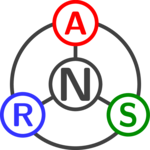
\includegraphics[height=1.5cm]{logo}
}

%https://tex.stackexchange.com/questions/55806/mindmap-tikzpicture-in-beamer-reveal-step-by-step
  \tikzset{
    invisible/.style={opacity=0},
    visible on/.style={alt={#1{}{invisible}}},
    alt/.code args={<#1>#2#3}{%
      \alt<#1>{\pgfkeysalso{#2}}{\pgfkeysalso{#3}} % \pgfkeysalso doesn't change the path
    },
  }


% https://tex.stackexchange.com/questions/446468/labels-with-arrows-for-an-equation
% https://tex.stackexchange.com/a/402466/121799
\newcommand{\tikzmark}[3][]{
\ifmmode
\tikz[remember picture,baseline=(#2.base)] \node [inner sep=0pt,#1](#2) {$#3$};
\else
\tikz[remember picture,baseline=(#2.base)] \node [inner sep=0pt,#1](#2) {#3};
\fi
}

\lstset{language=matlab,
                basicstyle=\scriptsize\ttfamily,
                keywordstyle=\color{blue}\ttfamily,
                stringstyle=\color{blue}\ttfamily,
                commentstyle=\color{gray}\ttfamily,
                morecomment=[l][\color{gray}]{\#}
              }

              
\begin{document}

\maketitle

% \begin{frame}
%   \frametitle{Second half of the semester}
%   \pause
%   Modules to be covered in the next 4 weeks: \\ \pause
%   \begin{enumerate}[<+->]\setcounter{enumi}{6}
%   \item Tree-based methods
%   \item Support Vector Machines (SVM)
%   \item Neural Networks
%   \item Unsupervised Learning
%     \begin{itemize}[<+->]
%     \item Principal components analysis (PCA)
%     \item Clustering analysis
%     \end{itemize}
%   \end{enumerate}

%   \pause

%   \textbf{Project}\pause
%   \begin{itemize}
%   \item Check Moodle for instructions; proposals due April 10
%   \end{itemize}
%   \pause

%   \medskip
  
%   \textbf{Final Exam}\pause
%   \begin{itemize}
%   \item Cumulative 24-hr open-book take-home exam.
%   \end{itemize}
% \end{frame}

\begin{frame}
  \frametitle{Outline for this lecture}\small
  \tableofcontents
\end{frame}

%\section{Introduction}
 
 
 
% \begin{frame}
%   \frametitle{Variable importance in random forests}

%   %   \begin{figure}[h!]
%   %     \centering
%   %     \visible<6->{\includegraphics[width=.75\textwidth, trim={4.5cm 8cm 4cm 4.4cm}, clip]{ESL15-5}}
%   %     \caption{}
%   % \end{figure}


% \end{frame}


% \begin{frame}
%   \frametitle{Introduction}
  
% \end{frame}
  

% \begin{frame}
%   \frametitle{Neural networks}
%   \pause

%   networks
% \end{frame}

\section{Introduction}
\begin{frame}
  \frametitle{Biological neuron}
  \pause


  \visible<2->{\begin{figure}[h!]
    \centering
    \includegraphics[width=.8\textwidth]{neuron}
    \caption{Biological neuron (Source: \url{https://cs231n.github.io/neural-networks-1/})}
  \end{figure}}

  \begin{itemize}[<+->]
  \item $\sim$86 billion neurons are found in the human nervous system
  \item These neurons are connected by 10$^{14}$ to $10^{15}$ synapses
  \item Each neuron receives input signals from its dendrites and outputs signals along a single axon
  \item The axon in turn connects to other neurons via synapses
  \end{itemize}
\end{frame}

\begin{frame}
  \frametitle{Computational neuron model}
  \pause
  \begin{figure}[h!]
    \centering

    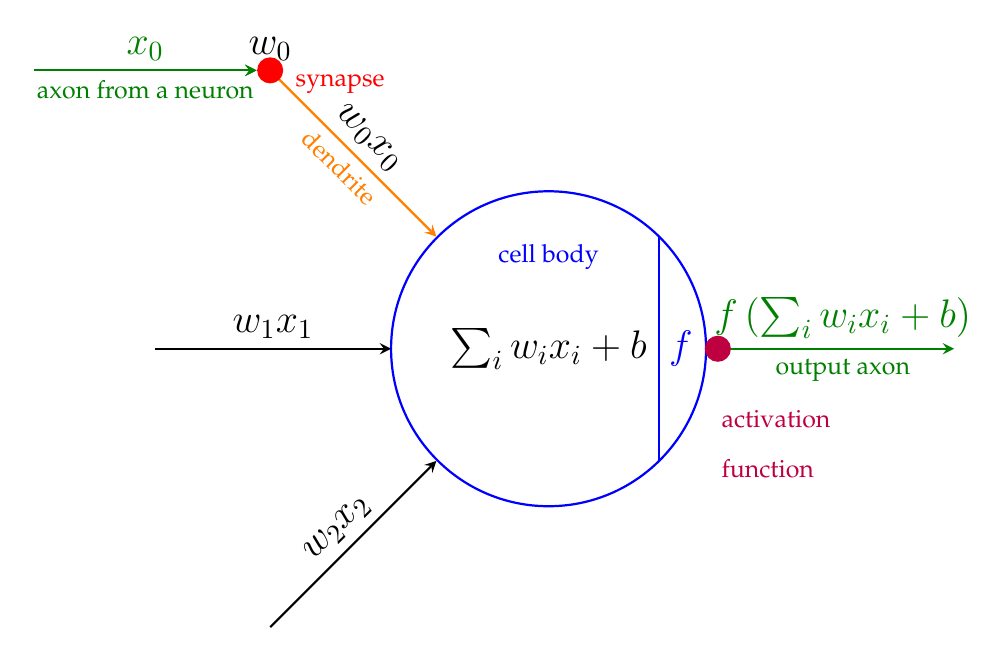
\begin{tikzpicture}[>=stealth,scale=1]
      \visible<13->{\begin{scope}
        \clip[radius=2cm] (0,0) circle;
        \draw[thick,blue] (1.4,-2) -- (1.4,2) node [right,pos=.5] {$f$};
      \end{scope}}
      \visible<12->{\node (O) at (0,0) {$\sum_i w_i x_i + b$ };}
      \visible<11->{\node[above=5mm of O,blue] {\small\normalfont cell body};}
      \visible<10->{\node[blue, thick, draw, circle,minimum width=4cm] at (O) (N) {} ;}
      \visible<14->{\node[circle,fill=purple,minimum width=1mm,xshift=1.5mm] (A) at (2,0) {};}
      \visible<15->{\node[below right of=A,text width=8ex, yshift=-.5cm,purple,] {\small\normalfont activation function};}
      \visible<16->{\draw[->, green!50!black,thick] (A) -- +(3,0) node[below,pos=.5] {\small\normalfont output axon};}
      \visible<17->{\path[->, green!50!black,thick] (A) -- +(3,0) node[above,pos=.5] {$f\lt(\sum_iw_ix_i + b\rt)$};}
      \visible<8->{\draw[->, thick] (-5,0) -- (-2,0) node[above,pos=.5] {$w_1x_1$};}
      \visible<9->{\draw[<-, thick] (N.225) -- (225:5cm) node [above,sloped,pos=.5] {$w_2x_2$};}
      \visible<6->{\draw[<-, thick,orange] (N.135) -- (135:5cm)   node[below,sloped,pos=.5] {\small \normalfont dendrite};}
      \visible<7->{\path[] (N.135) -- (135:5cm)  node[above,sloped,pos=.5] {$w_0x_0$};}
      \visible<4->{\path[] (N.135) -- (135:5cm)  node[opacity=1,circle,fill=red, minimum width=1mm] (W) {};
      \node[above] at (W) (S) {$w_0$};}
      \visible<5->{\node[below right,xshift=2mm,yshift=-2mm] at (S) {\rd \small\normalfont synapse};}
      \visible<2->{\draw[<-, thick,green!50!black ] (135:5cm) (W) -- +(-3,0) node[below,pos=.5] {\small\normalfont axon from a neuron};}
      \visible<3->{\draw[<-, thick,green!50!black ] (135:5cm) (W) -- +(-3,0) node[above,pos=.5] {$x_0$};}
      % \end{scope}
    \end{tikzpicture}
    
    %\caption{Computational neuron components}
  \end{figure}
  
\end{frame}

\begin{frame}
  \frametitle{Neural networks - basic ML terminology}
  \pause


  \begin{itemize}[<+->]
  \item $x_i$: \pause  signals traveling along axons (inputs)
  \item $w_i$: \pause  measure of synaptic strength, which is learned;\\ \pause
    \begin{itemize}[<+->]\item 
$w_i > 0 \rightarrow$ excitory influence
\item    $w_i <0 \rightarrow$ inhibitory influence
  \end{itemize}
  \item Dendrites carry signals $w_ix_i$ to the cell body, where they are summed.
  \item If the final sum $w_ix_i + b > t$ where $t$ is a threshold\footnote{intercept $b$ is referred to as the ``bias'' in ML literature},
   the neuron sends a spike along its axon (i.e.\ fires)
 \item Computationally, the firing rate of a neuron is represented by an \textbf{\pl activation function $f$}
 \item The output of a neuron is also called the \textit{\pl activation}
 \item   The output neurons have no activation function. Instead, they perform a final transformation of outputs from the penultimate layer
 \item  [Artificial] Neural networks (ANNs) are typically  modeled as connected layers of neuron in an acyclic graph (no loops).
  \item $N$-layer neural network (number of hidden layers $+$ output layer)
  \end{itemize}
\end{frame}


% \begin{frame}
%   \frametitle{Nomenclature}
%   \pause

%   [Artificial] Neural networks (ANNs) are modeled as connected layers of neuron in an acyclic graph (no loops).
  
%   \begin{itemize}[<+->]
%   \item ANNs are organized into layers of neurons (or ``units'')
%   \item Fully-connected layers are common
%   \item The basic ANN architecture with multiple hidden layers is called the \textbf{multilayer perceptron (MLP}
%   \item An ANN with only one hidden layer is called the \textbf{single layer perceptron}
%   \item $N$-layer neural network (number of hidden layers $+$ output layer)
%   \item The output neurons have no activation function. Instead, they perform a final transformation of outputs from the penultimate layer
%   \end{itemize}
% \end{frame}
% \begin{frame}
%   \frametitle{Examples of activation functions}
%   \pause
%   \begin{figure}[t!]
%     \begin{tikzpicture}[scale=1.7]
%       \begin{axis}[width=5cm,height=5.5cm,
%         ylabel=,
%         xlabel=$z$,ymin=-1.25,ymax=1.25,xmin=-5,xmax=5,
%         style={font=\tiny\normalfont},
%         legend style ={at={(1,.7)},anchor=west,align=left}
%         ]
%         \addplot[thick,blue,smooth] {1/(1+exp(-x))}; \addlegendentry{Logistic sigmoid: $\sigma(z)$}
%         \addplot[thick,red,smooth] {tanh(x)}; \addlegendentry{Hyperbolic tangent: $\tanh(z)$}
%         \addplot[thick,green,smooth,domain=-5:-0.001] {max(0,x)}; \addlegendentry{ReLU: $\max(0,z)$}
%         \addplot[thick,green,smooth,domain=0.001:5] {max(0,x)}; 
%         \end{axis}
%       \end{tikzpicture}
      
%     	% \caption[Sigmoidal activation functions.]{Common used activation functions include the logistic sigmoid $\sigma(z)$ and the hyperbolic tangent $tanh(z)$. More recently used activation functions are the softsign and the rectified hyperbolic tangent.}
%     	% \label{fig:sigmoid-tanh}
% \end{figure}
% \end{frame}







 


\begin{frame}[fragile]
  \frametitle{Three-layer neural network (with bias neurons)}
  \begin{figure}[h!]
    \centering
    \begin{neuralnetwork}[height=4]
    \newcommand{\x}[2]{$x_#2$}
    \newcommand{\y}[2]{$\hat{y}_#2$}
    \newcommand{\hfirst}[2]{\small $h^{(1)}_#2$}
    \newcommand{\hsecond}[2]{\small $h^{(2)}_#2$}
    \inputlayer[count=3, bias=true, title=I, text=\x]
    \hiddenlayer[count=4, bias=true, title=H1, text=\hfirst] \linklayers
    \hiddenlayer[count=3, bias=true, title=H2, text=\hsecond] \linklayers
    \outputlayer[count=2, title=O, text=\y] \linklayers
  \end{neuralnetwork}
\end{figure}

\pause
  \begin{itemize}[<+->]
  \item \textbf{Layers}: 3; \pause  \textbf{Hidden layers:} 2
  \item \textbf{Neurons}: 9
  \item \textbf{Learnable parameters:} $(4\times 4) + (5\times 3) + (4\times 2) = \pause 39$ weights
  \end{itemize}
  
\end{frame}





\begin{frame}
  \frametitle{Matrix operations in neural networks}
  \pause
%  The activation in the next layer can be constructed as a matrix operation as follows.\pause

  Given the activation vector ($m+1$ neurons) in the zeroth (input) layer:
  \begin{equation}
    a^{(0)} =   \begin{bmatrix}
    a_0^{0}\\[2mm]
    a_1^{0}\\[2mm]
    \vdots \\[2mm]
    a_m^{0}\\
    \end{bmatrix}
  \end{equation}
  \pause
  Then the activations in the next layer ($j+1$ neurons) are given by:\pause
  \begin{equation}
    a^{(1)}=
    \sigma\left(
    \boldsymbol{W}a^{0}+b
  \right)
  = \pause
  \sigma \left(
    \begin{bmatrix}
    w_{0,0} & w_{0,1} & \cdots & w_{0,k}\\
    w_{1,0} & w_{1,1} & \cdots & w_{1,k}\\
    \vdots & \vdots & \ddots & \vdots \\
    w_{j,0} & w_{j,1} & \cdots & w_{j,k}\\
    \end{bmatrix}
    \, 
    \begin{bmatrix}
    a_0^{0}\\
    a_1^{0}\\
    \vdots \\
    a_n^{0}\\
    \end{bmatrix}
    +
    \begin{bmatrix}
    b_0\\
    b_1\\
    \vdots \\
    b_n\\
    \end{bmatrix}
    \right)
  \end{equation}
  \pause
  Example: If Layer 1 had only two neurons, then the weight matrix $\bm W$ would have only 2 rows.
\end{frame}


\section{Training overview}
\begin{frame}
  \frametitle{Another look at the neuron}
  \pause
  Given the notation formalization, we revisit the neuron.\pause

  \begin{center}
  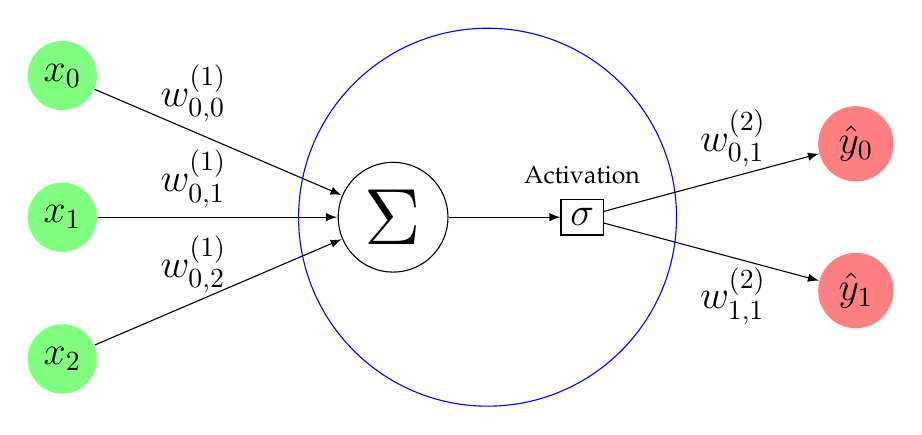
\begin{tikzpicture}[>=latex,scale=1.2]
\path
(0,0)     node[circle,draw,scale=2,inner sep=2pt] (S) {$\Sigma$}
% +(90:2.5) node[circle,draw,inner sep=2.5pt,opacity=0] (b) {}
%           node[above=1mm] {}
+(-3.5,1.5)  node[circle,fill=green!50]  (x1) {$x_0$}
+(-3.5,0)    node[circle,fill=green!50]  (x2) {$x_1$}
+(-3.5,-1.5) node[circle,fill=green!50]  (x3) {$x_2$}
(2,0)    node[draw] (g) {$\sigma$} node[above=3mm]{\small\normalfont Activation}
+(15:3)  node[circle,fill=red!50]  (y1) {$\hat{y}_0$}
+(-15:3) node[circle,fill=red!50]  (y2) {$\hat{y}_1$};
\draw[->] (S)--(g);
%\draw[->] (b)--(S);
\draw[->] (g)--(y1) node[pos=.6,above]{$w_{0,1}^{(2)}$};
\draw[->] (g)--(y2) node[pos=.6,below]{$w_{1,1}^{(2)}$};
\draw[->] (x1)--(S) node[pos=.4,above]{$w_{0,0}^{(1)}$};
\draw[->] (x2)--(S) node[pos=.4,above]{$w_{0,1}^{(1)}$};
\draw[->] (x3)--(S) node[pos=.4,above]{$w_{0,2}^{(1)}$};
\draw[blue] (1,0) circle(2);
\end{tikzpicture}
\end{center}

\end{frame}

\begin{frame}
  \frametitle{Neural network notation}
  \pause

  
  The {\bf \bl activation (output)} of a neuron is denoted:\pause
  \begin{equation}\bl
    \sigma(w_1a_1 + w_2a_2 + \cdots + w_n a_n + b) = \sigma(\sum w_ia_i + b) = \text{new neuron}
  \end{equation}
  \pause
  Further, we denote each activation as $a_{neuron}^{(layer)}$, e.g.\pause
  \begin{itemize}[<+->]
  \item $a_3^{(1)}$: fourth neuron in first layer (layers are counted from first hidden layer)
  \end{itemize}
  \pause

  \bigskip
  
  \begin{minipage}[t]{.47\linewidth}
  \textbf{\rd Weights} are denoted as $\rd w_{to,from}$, e.g.\pause
  \begin{itemize}[<+->]
  \item $w_{1,2}^2$: from neuron 3 to neuron 2 in second layer
  \item The superscript is not often used, as it is clear from the context which layer we are dealing with
  \end{itemize}
\end{minipage}  \pause
\begin{minipage}[t]{.47\linewidth}
  \begin{figure}[h!]
    \centering
    \includegraphics<9->[width=.8\textwidth]{nn-1-3}
  \end{figure}
\end{minipage}
\end{frame}


\begin{frame}
  \frametitle{Training a neural network}\pause
  
  % Let us describe a single hidden layer neural network using the following equations:\pause

  % \begin{align}
  %   Z_m &= \sigma(b_m + w_m^TX), \quad m = 1, \ldots, M \\
  %   T_k &= b_k + w_k^TZ, \quad k =1\ldots, K \\
  %   y_k(X) &= g_k(T), \quad k= 1,\ldots, K
  % \end{align}

  % \begin{itemize}[<+->]
  % \item $p$ is number of input units/neurons
  % \item $M$ is number of hidden units/neurons
  % \item $K$ is number of output units/neurons
  % \item Note: $w_m^TX = \sum_i w_{mi}x_i$
  % \item Total number of learnable parameters: $M(p+1) + K(M+1)$ weights
  % \end{itemize}

  \begin{itemize}[<+->]
  \item A neural network is trained or fitted by \textit{learning} the optimal values of the weights.
  \item This learning is done via optimization (e.g.\ gradient descent)
  \item Gradient descent: \pause
    \begin{equation}
      w^{\text{new}} = w^{\text{old}} - \eta \pd{C}{w^{\text{old}}}
    \end{equation}
    \pause
    where:
    \begin{itemize}[<+->]
    \item $\eta$ is the learning rate
    \item $C$ is the cost function (e.g.\ residual sum of squares):\pause
      \begin{equation}
        C = \sum_{i=1}^n (y_i - \hat y_i)^2
      \end{equation}
    \item $w$ the weight
  \end{itemize}

  \item In neural networks, the gradients are computed via \textbf{\bl backpropagation}
  \end{itemize}
\end{frame}
 

\begin{frame}
  \frametitle{Neural network loss function}
  \pause
  Given $k$ output neurons and $i$ observations (where $\theta$ represents the weights and $f_k$ the output),
  we can compute the loss functions as follows. \pause

  \medskip
  
  \textbf{For regression:}
  \begin{equation}
    R(\theta) = \sum_{k=1}^K\sum_{i=1}^n(y_{ik} - f_k(x_i))^2
  \end{equation}

  \pause

  \medskip
  
  \textbf{For classification}, we use the cross-entropy (deviance):\pause
  \begin{equation}
    R(\theta) = - \sum_{i=1}^n\sum_{k=1}^Ky_{ik} \log f_k(x_i))
  \end{equation}

  \pause

  In modern ML terminology, this loss is usually referred to as a cost function $C$. \pause

  Thus, we can write, where $k=1$:

  \begin{equation}
    C = \sum_{i=1}^n (y_i - \hat y_i)^2
  \end{equation}
\end{frame}





\begin{frame}
  \frametitle{Summary of backpropagation}\pause

  \begin{enumerate}[<+->]
  \item Fix initial weights $w^{(l),0}$, $b^{(l),0}$ and perform a forward sweep/pass through the network computing the activations $a$ (outputs) of each layer $l$ as:\pause
    \begin{equation}
      a^{(l)} = \sigma(\bm W^{(l)} a^{(l-1)} + b^{(l)})
    \end{equation}
  \item At the output layer, we compute the cost function $C$ (what we want to minimize)
  \item Then, we {\it backpropagate} the errors through each layer in order to compute the gradients $\pd{C}{w^{(l)}}$, $\pd{C}{b^{(l)}}$ \pause
    and  weight updates  $w^{(l),r+1}$ and $b^{(l),r+1}$
\item Repeat the forward and backward passes until cost is sufficiently minimized
  \end{enumerate}
  
\end{frame}


\begin{frame}
  \frametitle{Example: backpropagation for 3-layer network}
  \pause
%  Consider the ANN below. What are the cost function gradients? \pause
\visible<2->{  \begin{figure}[h!]
    \centering
    \includegraphics[width=.6\textwidth]{4layer-nn}
  \end{figure}
}
\pause
\vspace{-2ex}
\begin{align}
 \pd{C}{w^{(3)}} &=  {\rd \pd{C}{a^{(3)}}\pd{a^{(3)}}{z^{(3)}}}\pause \pd{z^{(3)}}{w^{(3)}}\\\pause
\pd{C}{w^{(2)}} &=  {\rd \pd{C}{a^{(3)}}\pd{a^{(3)}}{z^{(3)}}} \pause {\bl \pd{z^{(3)}}{a^{(2)}}\pd{a^{(2)}}{z^{(2)}}} \pause                   
                    \pd{z^{(2)}}{w^{(2)}}\\\pause  
\pd{C}{w^{(1)}} &=  {\rd \pd{C}{a^{(3)}}\pd{a^{(3)}}{z^{(3)}}} \pause {\bl \pd{z^{(3)}}{a^{(2)}}\pd{a^{(2)}}{z^{(2)}}} \pause                   
                    \pd{z^{(2)}}{a^{(1)}}                          
                    \pd{a^{(1)}}{z^{(1)}}\pd{z^{(1)}}{w^{(1)}}
\end{align}
\end{frame}

 \begin{frame}
  \frametitle{Batch learning}
  The gradient descent method was described without referencing the observations. \pause

  \medskip

  In reality, the forward and backward passes are performed for each observation in the training set, with parameter updates obtained by
  \textbf{\bl averaging} the gradients: \pause

  \begin{align}
    w^{(l), r+1}  &= \pause  w^{(l),r} - \pause \eta{\bl  \fr1n \sum_{i=1}^n}\pd{C_i}{w^{(l)}}  \\\pause
    b^{(l), r+1}  &=  \pause b^{(l),r} - \pause \eta {\bl \fr1n \sum_{i=1}^n} \pd{C_i}{b^{(l)}}  
  \end{align}

  \pause

  This approach is called \textbf{\bl batch learning}. \pause

  \begin{itemize}[<+->]
  \item One sweep through all the training observations is called an \textit{epoch}
  \item In batch learning, only one update results from a training epoch
  \item Thus, several epochs are required for convergence
  \end{itemize}
\end{frame}

\begin{frame}
  \frametitle{Stochastic gradient descent}
  \pause

  In standard gradient descent (batch learning), the updates are performed only after the gradient is computed for \textit{all} training observations.

  \pause

  \medskip
  
  The stochastic gradient descent approach approximates the gradient using a {\rd randomly selected}  observation: \pause

    \begin{align}
    w^{(l), r+1}  &= \pause  w^{(l),r} - \pause \eta \pd{C_{\rd i}}{w^{(l)}}  \\\pause
    b^{(l), r+1}  &=  \pause b^{(l),r} - \pause \eta  \pd{C_{\rd i}}{b^{(l)}}  
  \end{align}

  \pause

  \begin{itemize}[<+->]
  \item Each iteration over observation $i$ results in a weight/bias update
  \item Thus, one sweep through the entire training set (an epoch) produces $n$ updates
  \end{itemize}
  \pause
  This procedure is also known as \textbf{\rd online learning}
\end{frame}

\begin{frame}
  \frametitle{Mini-batch learning}
  \pause
  To introduce stability, we can compute weight updates over a \textit{\pl subset} of training observations

  \begin{enumerate}[<+->]
  \item Randomly partition the training set into $M$ mini-batches, each with $m$ observations
  \item Perform a forward and backward pass through each mini-batch to update the weights:\pause
      \begin{align}
    w^{(l), r+1}  &= \pause  w^{(l),r} - \pause \eta{\pl  \fr1m \sum_{i=1}^m} \pd{C_{\pl i}}{w^{(l)}}  \\\pause
    b^{(l), r+1}  &=  \pause b^{(l),r} - \pause \eta{\pl  \fr1m \sum_{i=1}^m}  \pd{C_{\pl i}}{b^{(l)}}  
  \end{align}
  \pause
  Thus, for each iteration, average the gradient over a \textit{\pl mini-batch} of $m$ observations
\item Repeat step 2 until convergence
  \end{enumerate}  
\end{frame}

\begin{frame}
  \frametitle{Performance and robustness considerations }
  \pause
  \begin{itemize}[<+->]
  \item Online learning is more efficient for very large datasets
  \item In practice, mini-batch learning is employed, as batch sizes (usually, $m=16$ or $m=32$) can be chosen to take advantage of parallel computing architectures
  \item An \textit{\bf \rd adpative} learning rate $\eta$ can guarantee convergence, e.g. $\rd \eta_r = \fr1r$
  \item \textit{Overfitting} can be mitigated via \textbf{\bl weight decay} (regularization of weights):\pause
    \begin{equation}\bl 
      C \leftarrow \pause C + \la J = \pause C + \la\lt(\sum w^2 + \sum b^2\rt)
    \end{equation}
    \pause where $\la$ is tuning parameter estimated via cross-validation\\
    \textit{Early stopping} and \textit{dropout} are also used.
  \item Input \textbf{standardization} (mean zero, SD 1) is recommended for consistent weight initialization and regularization
  \item Weights/biases are initialized to \textit{small} values near 0 for better performance
  \item Cost function $C$ is nonlinear and nonconvex; other optimization approaches (e.g.\ conjugate gradient) can provide faster convergence compared to
    stochastic gradient descent
  \end{itemize}
\end{frame}

%\section{Further architectures}
\begin{frame}
  \frametitle{Other types of neural networks}
  \pause

  The standard ANN architecture (MLP) we have studied is also called the feed-forward network.

  \medskip
  
  Other architectures have been shown to give better performance for various applications: \pause

  \medskip
  \begin{itemize}[<+->]
  \item Recurrent neural networks (RNNs): time-series forecasting

  \item Convolutional neural networks (CNNs): image classification

  \item Long short-term memory networks (LSTMs): time-series, pattern identification, etc.
  \end{itemize}
\end{frame}

\section{Convolutional NNs}
\begin{frame}
  \frametitle{The convolutional neural network (CNN)}
  \pause

  \begin{itemize}
  \item Motivated by the image recognition process of the brain's visual cortex.

  \item Groundbreaking study on cats revealed the importance of \textit{local receptive fields} for activating neurons
    in the visual cortex. (Hubel \& Wiesel, 1958; 1959)

  \item Earliest neural network for image recognitron introduced: \textit{neocognitron} (Fukushima, 1980)

  \item Milestone: introduction of \textit{LeNet-5} architecture for handwritten digit recognition (Yann LeCun et al., 1998)
  \end{itemize}
  
\end{frame}

\begin{frame}
  \frametitle{Building blocks of a CNN}

  \begin{itemize}
  \item \textbf{Input layer:} the image to be classified 
  \item \textbf{Convolutional layer:} represents the action of a filter transmitting signals (features) from various
    portions (receptive fields) of the preceding layer. The size of the receptive field is specified by the
    \textit{convolutional kernel}. Each layer can have multiple feature maps representing different filters.
  \item \textbf{Pooling layer:} subsamples signals from preceding layer to reduce dimensionality and extract dominant
    features (subsample space determined by kernel size)
  \item \textbf{Dense layer:} neuron outputs are flattened and fully connected %(usually with decreasing number of neurons)
  \item \textbf{Output layer:} neurons equal to number of classes; with softmax activation
  \end{itemize}

  \begin{center}
    \includegraphics[width=.6\textwidth]{cnn-ex1}
  \end{center}

  {\tiny Source: \url{https://neurdiness.wordpress.com/2018/05/17/deep-convolutional-neural-networks-as-models-of-the-visual-system-qa/}}

  
\end{frame}

\begin{frame}
  \frametitle{Training hyperparameters in a CNN}
  Several decisions must be made in selecting hyperparameters for training a CNN.

  \begin{itemize}
  \item Number of convolutional layers and feature maps in each layer
  \item Convolutional kernel size
  \item Stride length (spacing of filters)
  \item Choice of pooling function (max, average, etc)
  \item Number of dense layers
  \item Activation function in each layer (ReLU, tanh, etc)
  \end{itemize}

  Various high-performing architectures have been developed in recent years that can be adapted for other problems.

  Training the network involves finding the weights for the various layers (using mini-batch gradient descent or other variants)
\end{frame}

\begin{frame}
  \frametitle{Another CNN example}
  \begin{center}
    \includegraphics[width=.9\textwidth]{cnn-ex2}
  \end{center}
  {\tiny Source: \url{https://towardsdatascience.com/mnist-handwritten-digits-classification-using-a-convolutional-neural-network-cnn-af5fafbc35e9}}
\end{frame}

\section{AI for Tree Risk}
\begin{frame}
  \frametitle{Automating tree risk prediction using AI}

  \begin{itemize}
  \item \textbf{Objective:}  Automate tree risk classification using a convolutional neural network?
  \item \textbf{Question 1:} Can we elicit the visual features from a trained network that indicate various levels of risk?
  \item \textbf{Question 2:} Can we map estimated CNN weights to structural relationships governing tree stability?
  \item \textbf{Question 3:} How well can a trained CNN be transferred to another set of images and perform similarly well for risk prediction?
  \item \textbf{Question 4:} How can this process be adapted for Google Maps images (or drone photography)?
  \end{itemize}
\end{frame}

\begin{frame}
  \frametitle{CNN Model 1}
  \begin{itemize}
  \item Cropped and resized images to $108\times 108\times 1$ (grayscale)
  \item Binary classification; 103 probable/possible and 259 improbable
  \item Used a simple architecture (5 convolutional layers, 2 hidden dense layers, 1 output layer)
%     \begin{quote}\tiny
%  \begin{verbatim}
% model = models.Sequential([
%     layers.Conv2D(64, 7, activation="relu", padding="same", input_shape = input_image_shape),
%     layers.MaxPooling2D(2),
%     layers.Conv2D(128, 3, activation="relu", padding="same"),
%     layers.Conv2D(128, 3, activation="relu", padding="same"),
%     layers.MaxPooling2D(2),
%     layers.Conv2D(256, 3, activation="relu", padding="same"),
%     layers.Conv2D(256, 3, activation="relu", padding="same"),
%     layers.MaxPooling2D(2),
%     layers.Flatten(),
%     layers.Dense(128, activation="relu"),
%     layers.Dropout(0.5),
%     layers.Dense(64, activation="relu"),
%     layers.Dropout(0.5),
%     layers.Dense(2, activation="softmax")
% ])
% \end{verbatim}
%        \end{quote}
  \item Validation accuracy: 74\% (10 epochs)
  \item Increasing input image size to  $216\times 216$ worsens outcome with accuracy of 68\%
  \item If the stride in the first convolutional layer is increased to 2 (with the higher resolution), this does not improve the result.
  \item However, with a stride of 2 and $108\times 108$ image resolution, we obtain a validation accuracy of 77\%.
  \end{itemize}
\end{frame}

\begin{frame}
  \frametitle{CNN Model 2}

  \begin{itemize}
  \item Images are cropped but not converted to grayscale.
  \item Three classes: 40 probable, 63 possible , 259 improbable
  \item CNN architecture unchanged
  \item Validation accuracy: 74\% (10 epochs)        
  \end{itemize}
\end{frame}
\appendix
\section{Backpropagation}

\begin{frame}
  \frametitle{Equation summary: outer layer}
  \pause
  At the outer layer $L$ (without indexing by neuron):\pause
  \begin{align}
    z^{(L)} &= w^{(L)} \times a^{(L-1)} + b^{(L)} \\\pause
    a^{(L)} &= \sigma(z^{(L)}) \\\pause
    C &= (a^{(L)}  - y)^2
  \end{align}
  \pause
  
  The gradient of the cost function with respect to $w^{(L)}$ is:\pause
  \begin{equation}
    \frac{\partial C}{\partial w^{(L)}}
    =\pause
    \frac{\partial C}{\partial a^{(L)}}
    \frac{\partial a^{(L)}}{\partial z^{(L)}}
    \frac{\partial z^{(L)}}{\partial w^{(L)}}
    =\pause
    2 \left(a^{(L)} - y \right) \sigma' \left(z^{(L)}\right) a^{(L-1)}
  \end{equation}
  \pause
  Thus, we see that this gradient depends on the activation from the previous layer $a^{(L-1)}$. \pause Also wrt to the bias:
  \begin{equation}
    \pd{C}{b^{(L)}} = \pause \pd{C}{a^{(L)}}\pd{a^{(L)}}{z^{(L)}}\pd{z^{(L)}}{b^{(L)}} =\pause 2\lt(a^{(L)} - y\rt)\sigma'(z^{(L)})(1)
  \end{equation}
\end{frame}

\begin{frame}
  \frametitle{Updating weights}
  \pause
  We can then update the weights for the last layer for the next iteration $r+1$:\pause
  \begin{align}
    w^{(L), r+1}  &=  w^{(L),r} - \eta \pd{C}{w^{(L)}}  \\\pause
    b^{(L), r+1}  &=  b^{(L),r} - \eta \pd{C}{b^{(L)}}  
  \end{align}
  \pause
  To update the weights for layer $L-1$, we need to find the gradients $\pd{C}{w^{(L-1)}}$ and $\pd{C}{b^{(L-1)}}$.

  \pause

  \medskip
  
  Using the chain rule again, we write:\pause
  \begin{align}
    \pd{C}{w^{(L-1)}} &= {\rd \pd{C}{a^{(L-1)}}}\pd{a^{(L-1)}}{z^{(L-1)}}\pd{z^{(L-1)}}{w^{(L-1)}} \\\pause
    \pd{C}{b^{(L-1)}} &= {\rd \pd{C}{a^{(L-1)}}}\pd{a^{(L-1)}}{z^{(L-1)}}\pd{z^{(L-1)}}{b^{(L-1)}} 
  \end{align}
\end{frame}

\begin{frame}
  \frametitle{Backward pass}
  \pause
  But we recall that $C$ is not \textit{explicitly} dependent on $a^{(L-1)}$ as $C = (a^{(L)} - y)^2$.
  \pause

  However, it is \textit{implicitly} dependent, since\pause
  \begin{equation}
    C \propto a^{(L)},
  \end{equation}
  \pause
  \begin{equation}
    a^{(L)} \propto z^{(L)} 
  \end{equation}
  \pause
  and\pause
  \begin{equation}
    z^{(L)} \propto a^{(L-1)}
  \end{equation}
  \pause
  
  So, we use the chain rule to expand $\pd{C}{a^{(L-1)}}$ as follows:\pause
  \begin{equation}\rd
    \pd{C}{a^{(L-1)}} = \pause \pd{C}{a^{(L)}}\pd{a^{(L)}}{z^{(L)}}\pd{z^{(L)}}{a^{(L-1)}}
  \end{equation}
\end{frame}

\begin{frame}
  \frametitle{Backward pass (cont.)}
  \pause
  We can then expand the cost function gradient wrt to weights for layer $L-1$ as:\pause
  \begin{align}
    \pd{C}{w^{(L-1)}} &= {\rd \pd{C}{a^{(L-1)}}}\pd{a^{(L-1)}}{z^{(L-1)}}\pd{z^{(L-1)}}{w^{(L-1)}} \pause
                        = {\rd \pd{C}{a^{(L)}}\pd{a^{(L)}}{z^{(L)}}\pd{z^{(L)}}{a^{(L-1)}}} \pd{a^{(L-1)}}{z^{(L-1)}}\pd{z^{(L-1)}}{w^{(L-1)}} \\[2mm]\pause
        \pd{C}{b^{(L-1)}} &= {\rd \pd{C}{a^{(L-1)}}}\pd{a^{(L-1)}}{z^{(L-1)}}\pd{z^{(L-1)}}{b^{(L-1)}} 
                            = {\rd \pd{C}{a^{(L)}}\pd{a^{(L)}}{z^{(L)}}\pd{z^{(L)}}{a^{(L-1)}}} \pd{a^{(L-1)}}{z^{(L-1)}}\pd{z^{(L-1)}}{b^{(L-1)}} 
  \end{align}

  \pause

  Once these gradients are computed, we update the weights for the $r+1$th iteration using: \pause
   \begin{align}
    w^{(L-1), r+1}  &= \pause  w^{(L-1),r} - \pause \eta \pd{C}{w^{(L-1)}}  \\\pause
    b^{(L-1), r+1}  &=  \pause b^{(L-1),r} - \pause \eta \pd{C}{b^{(L-1)}}  
  \end{align}
\end{frame}

\begin{frame}
  \frametitle{Summary: forward pass}
  \begin{enumerate}[<+->]
  \item Initialize weights and biases: $w^{(l),0}$, $b^{(l),0}$
  \item Perform forward pass to compute activations:
    \begin{align}
      z^{(l),0} &= w^{(l),0} \times a^{(l-1),0} + b^{(l),0} \\\pause
    a^{(l)} &= \sigma(z^{(l),0}) 
    \end{align}
    \pause
    At output layer:
    \begin{align}      
      z^{(L),0} &= w^{(L),0} \times a^{(L-1),0} + b^{(L),0} \\\pause
      a^{(L),0} &= \sigma(z^{(L),0}) \\
      C &= (a^{(L),0}  - y)^2
    \end{align}
  \end{enumerate}
\end{frame}

\begin{frame}
  \frametitle{Summary: backward pass---outer layer }
  \begin{enumerate}[<+->]\setcounter{enumi}{2}
  \item Backward pass, outer layer $(L)$:\pause
    \begin{enumerate}[<+->]
    \item Compute gradients: \pause
      \begin{align}
      \pd{C}{w^{(L)}} &= \pause \pd{C}{a^{(L)}}\pd{a^{(L)}}{z^{(L)}}\pd{z^{(L)}}{w^{(L)}}\\\pause
      \pd{C}{b^{(L)}} &= \pause \pd{C}{a^{(L)}}\pd{a^{(L)}}{z^{(L)}}\pd{z^{(L)}}{b^{(L)}}\pause
      \end{align}
    \item Update weights: \pause
      \begin{align}
        w^{(L), 1}  &=  w^{(L),0} - \eta \pd{C^0}{w^{(L)}}  \\\pause
      b^{(L), 1}  &=  b^{(L),0} - \eta \pd{C^0}{b^{(L)}}  
      \end{align}
  \end{enumerate}
  \end{enumerate}
\end{frame}

\begin{frame}
  \frametitle{Summary: backward pass---last hidden layer}
  \begin{enumerate}[<+->]\setcounter{enumi}{2}
  \item Backward pass, layer $(L-1)$:\pause
    \begin{enumerate}[<+->]\setcounter{enumii}{2}
    \item Compute gradients: \pause
    \begin{align}
      \pd{C}{w^{(L-1)}} &=  \pd{C}{a^{(L)}}\pd{a^{(L)}}{z^{(L)}}\pd{z^{(L)}}{a^{(L-1)}}  \pd{a^{(L-1)}}{z^{(L-1)}}\pd{z^{(L-1)}}{w^{(L-1)}}\\\pause
      \pd{C}{b^{(L-1)}} &=   \pd{C}{a^{(L)}}\pd{a^{(L)}}{z^{(L)}}\pd{z^{(L)}}{a^{(L-1)}} \pd{a^{(L-1)}}{z^{(L-1)}}\pd{z^{(L-1)}}{b^{(L-1)}}
    \end{align}
    \pause
  \item Update weights: \pause
    \begin{align}
      w^{(L-1), 1}  &= \pause  w^{(L-1),0} - \pause \eta \pd{C}{w^{(L-1)}}  \\\pause
      b^{(L-1), 1}  &=  \pause b^{(L-1),0} - \pause \eta \pd{C}{b^{(L-1)}}  
    \end{align}
  \end{enumerate}
  \end{enumerate}
\end{frame}

\begin{frame}
  \frametitle{Summary: backward pass---second-to-last hidden layer}
  \begin{enumerate}[<+->]\setcounter{enumi}{2}
  \item Backward pass, layer $(L-2)$:\pause
    \begin{enumerate}[<+->] \setcounter{enumii}{4}
    \item Compute gradients: \pause
    \begin{align}
      \pd{C}{w^{(L-2)}} &=  \pd{C}{a^{(L)}}\pd{a^{(L)}}{z^{(L)}}\pd{z^{(L)}}{a^{(L-1)}} \pause
                        \pd{a^{(L-1)}}{z^{(L-1)}}\pd{z^{(L-1)}}{a^{(L-2)}} \pause
                        \pd{a^{(L-2)}}{z^{(L-2)}}\pd{z^{(L-2)}}{w^{(L-2)}}\\\pause
      \pd{C}{b^{(L-2)}} &=   \pd{C}{a^{(L)}}\pd{a^{(L)}}{z^{(L)}}\pd{z^{(L)}}{a^{(L-1)}} \pause
                        \pd{a^{(L-1)}}{z^{(L-1)}}\pd{z^{(L-1)}}{a^{(L-2)}} \pause
                        \pd{a^{(L-2)}}{z^{(L-2)}}\pd{z^{(L-2)}}{b^{(L-2)}}\\\pause
    \end{align}
    \pause
  \item Update weights: \pause
    \begin{align}
      w^{(L-2), 1}  &= \pause  w^{(L-2),0} - \pause \eta \pd{C}{w^{(L-2)}}  \\\pause
      b^{(L-2), 1}  &=  \pause b^{(L-2),0} - \pause \eta \pd{C}{b^{(L-2)}}  
    \end{align}
  \end{enumerate}
  \end{enumerate}
\end{frame}


\begin{frame}
  \frametitle{Summary: backward pass---first hidden layer}
  \begin{enumerate}[<+->]\setcounter{enumi}{2}
  \item Backward pass, layer $(1)$:\pause
        \begin{enumerate}[<+->] \setcounter{enumii}{4}
    \item Compute gradients: \pause
    \begin{align}
      \pd{C}{w^{(1)}} &=  \pd{C}{a^{(L)}}\pd{a^{(L)}}{z^{(L)}}\pd{z^{(L)}}{a^{(L-1)}}\pd{a^{(L-1)}}{z^{(L-1)}} \pause
                          \pause\cdots  
                          \pd{z^{(2)}}{a^{(1)}}                          
                        \pd{a^{(1)}}{z^{(1)}}\pd{z^{(1)}}{w^{(1)}}\\\pause
      \pd{C}{b^{(1)}} &=  \pd{C}{a^{(L)}}\pd{a^{(L)}}{z^{(L)}}\pd{z^{(L)}}{a^{(L-1)}}\pd{a^{(L-1)}}{z^{(L-1)}} \pause
                          \pause\cdots  
                          \pd{z^{(2)}}{a^{(1)}}                          
                        \pd{a^{(1)}}{z^{(1)}}\pd{z^{(1)}}{b^{(1)}}\\\pause
    \end{align}
    \pause
  \item Update weights: \pause
    \begin{align}
      w^{(1), 1}  &= \pause  w^{(1),0} - \pause \eta \pd{C}{w^{(1)}}  \\\pause
      b^{(1), 1}  &=  \pause b^{(1),0} - \pause \eta \pd{C}{b^{(1)}}  
    \end{align}
  \end{enumerate}
  \end{enumerate}
\end{frame}
% \section{Summary}
% \begin{frame}[fragile]
%   \frametitle{Summary}
%   \pause
%   Today, we considered an introduction to neural networks. We will finalize this on Friday with real examples.
%   \begin{itemize}[<+->]
%   \item For now, you may play around with \href{http://playground.tensorflow.org}{\bl \bf this}
%     \item Reading: ESL 11.3 -- 11.6 (complete before next lecture); you will notice differences in notation used.
%   \end{itemize}
% \end{frame}

% \begin{frame}
%   \frametitle{Reading}\pause
%   Today's lecture:\pause
  
% \begin{itemize}[<+->]
% \item Support vector machines: ISLR 9.3, 9.4; ESL 12.3.1
% \item 
%   % \item Boosting: ESL 10 (Very dense chapter. You may want to focus on 10.1--10.3, 10.7, 10.10, 10.13, 10.14.)
% \end{itemize}
% \pause
% \bigskip
  

% \end{frame}
 
%http://www.di.fc.ul.pt/~jpn/r/rbf/rbf.html
\end{document}

%%% Local Variables:
%%% mode: latex
%%% TeX-master: t
%%% End:
